\section{Metodología}\label{metodologia}

\subsection{Fuerza Bruta}

La técnica de \textbf{fuerza bruta} consiste en recorrer \textbf{todo} el espacio de soluciones en busca de aquellas factibles u óptimas. En este caso, el conjunto de soluciones está compuesto por todas las subsecuencias de $L$. Por ejemplo, si $L=[1,2,3]$ con $b=[20,15,30]$, $c=[10, 15, 20]$ y $M=30$ todas las subsecuencias posiblen son $[], [1], [2], [3], [1,2], [1,3], [2,3], [1,2,3]$ y las soluciones factibles son $[1], [2], [3], [1,3]$.

La idea del algoritmo \ref{alg:fuerza_bruta} es generar de forma recursiva las soluciones recorriendo todos los locales, pudiendo elegir incluir o no cada local en cada paso. Al contar con todo el espacio de soluciones, se recorre cada una para determinar si es factible y, en caso de serlo, se devuelve su beneficio total. Luego se selecciona alguna de las óptimas dentro del conjunto de soluciones factibles.

En la Fig. \ref{fig:ejemplo_fuerza_bruta} se puede observar un ejemplo del árbol de recursión generado para la instancia detallada más arriba. Cada nodo intermedio representa una solución parcial, es decir, la solución al problema considerando hasta el local \textit{i}-ésimo. Las hojas representan todas las soluciones posibles. La solución óptima se colorea con verde, las demás soluciones factibles, con azul y las soluciones no factibles, con rojo. La solución al problema analizado se obtiene llamando a $FB(L, n, M, vecindad, 0)$ donde $vecindad$ es un vector de \textit{boolean} inicializado en cada posición en \textit{False}.

La correctitud del algoritmo proviene del hecho de que se recorre \textit{todo} el espacio de soluciones, dado que para cada local de $L$ se generan dos ramas, si se considera para la subsecuencia o no. Y al llegar a las hojas se filtran las soluciones que no sean óptimas o factibles.

El algoritmo genera y recorre de forma completa en todos los casos un árbol de backtracking de $O(2^n)$ nodos. En cada uno se realizan operaciones de tiempo constante excepto en las hojas, en las cuales se realizan los chequeos de factibilidad que son $O(n)$, ya que iteran todo el vector de vecinos. Por lo tanto, la complejidad temporal del algoritmo es $O(2^n \times n)$. Se puede observar que frente a cualquier instancia el algoritmo se comportará de igual manera, dado que genera el mismo tipo de árbol con la misma cantidad de nodos, es por ello que el conjunto de instancias del peor caso es igual al del mejor caso.

% Algoritmo descriptivo de FB
\begin{algorithm}
    \begin{algorithmic}[1]
        \Function{FB}{$locales$, $n$, $M$, $vecindad$, $i$}
            \If{i = n + 1}
                \State $beneficio \gets 0$
                \State $contagio \gets 0$
                \For {j in [1..n]}
                    \If{$j \neq n \wedge vecindad[j] = True \wedge vecindad[j+1] = True$} \Comment{Hay dos vecinos consecutivos}
                        \State{\textbf{return} instancia inválida}
                    \EndIf
                    
                    \If{$petenencia[j] = True$} \Comment{El local actual pertence}
                        \State $beneficio \gets beneficio + b_j$
                        \State $contagio \gets contagio + c_j$
                    \EndIf
                    
                    \If{$contagio > M$}
                        \State{\textbf{return}  instancia inválida}
                    \EndIf
                    
                \EndFor
                \State{\textbf{return} $beneficio$}
            \Else 
                \State \textcolor{gray}{\textit{Usamos $(var \gets value)$ como algo que devuelve $var$ modificado por simplicidad.}}
                \State $\begin{aligned}[t]
                    \text{\textbf{return }} max(&FB(locales,\ n,\ M,\ (vecindad[i] \gets False),\ i+1),\\
                    &FB(locales,\ n,\ M - c_i,\ (vecindad[i] \gets True),\ i+1)&
                \end{aligned}$
            \EndIf
        \EndFunction
    \end{algorithmic}
    \caption{Algoritmo de $Fuerza$ $Bruta$ para NPM.}
    \label{alg:fuerza_bruta}
\end{algorithm}

% Gráfico con árbol de recursión de FB
\begin{figure}[H]
    \centering
    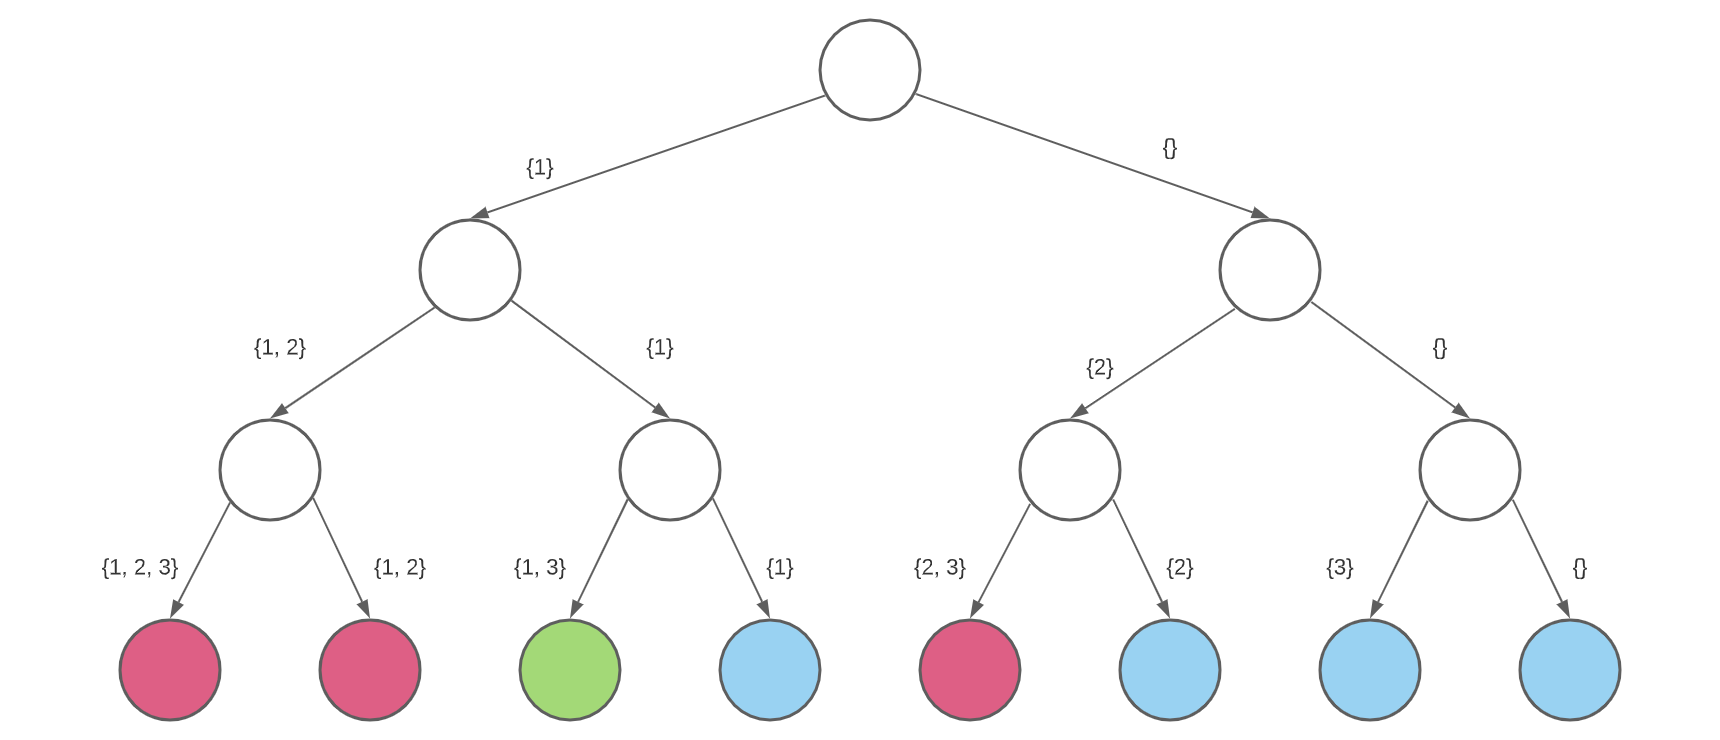
\includegraphics[scale=0.15]{img/Tree-Locales.png}
    \caption{Ejemplo de ejecución del Algoritmo~\ref{alg:fuerza_bruta} para $L=[1,2,3]$ con $b=[20,15,30]$, $c=[10, 15, 20]$ y $M=30$. En rojo las soluciones no factibles, en azul las factibles y en verde la solución óptima $\{1, 3\}$. En cada paso se agrega o no cada local al subconjunto, el cual se marca en las aristas.}
    \label{fig:ejemplo_fuerza_bruta}
\end{figure}

\subsection{Backtracking}

El algoritmo de \textit{backtracking} recorre un árbol para generar las soluciones posibles de manera similar a FB. La diferencia radica en la presencia de \textit{podas}, es decir, reglas que permiten evitar explorar todo el espacio de soluciones omitiendo recorrer ciertas ramas basado en algún criterio. Se dividen en dos tipos: \textit{factibilidad} y \textit{optimalidad}.

\begin{itemize}
    \item \textbf{Factibilidad.} Dada una solución parcial $S'$ representada por un nodo intermedio $n_0$ que cuenta con un contagio acumulado $m=\sum S'_c$ y el vector de vecindad en estado $V'$. Como para todo local $L_i$ tenemos valores de contagio positivos, si $m>M$ entonces no tiene sentido continuar extendiendo $S'$ porque en todos los casos el contagio final excederá $M$. Además, si en $V_i$ tenemos las últimas dos posiciones del vector indicando que están presentes $L_{i+1}$ y $L_{i+2}$, cualquiera de las soluciones finales tendrá dos vecinos colindantes y no será factible. En cualquiera de los dos casos, se puede evitar continuar recorriendo el subárbol formado a partir del eje $n_0$ y así reducir el número de operaciones. Se puede observar el pseudocódigo en el algoritmo \ref{alg:bactkracking}
    \item \textbf{Optimalidad.} Dada una solución parcial $S'$ representada por un nodo intermedio $n_i$ con beneficio $b=\sum S'_b$. Se cuenta con la solución factible con beneficio máximo $B$ hasta el momento. En cada nodo se calcula $b_r$, beneficio que se puede obtener al agregar a todos los locales por recorrer. Finalmente, si $b + b_r\le B$ cualquier decisión que se tome a continuación en el subárbol llevará a una solución al menos tan buena como la ya conocida. Por lo tanto, se puede podar esa rama y evitar cálculos innecesarios. En el algoritmos \ref{alg:bactkracking} se actualiza la variable de $maxB$ cada vez que se encuentra una solución factible y se evalúa la regla de la poda. Además, se agrega una pequeña variación que precalcula los valores de $b_r$ para cada nodo y los almacena en una caché. La única diferencia entre ambos es cómo se implementa $maximoBeneficioRestante$ de la línea \ref{alg:bt-max-restante}. 
\end{itemize}

% Algoritmo descriptivo de BT
\begin{algorithm}
    \begin{algorithmic}[1]
        \Function{$BT$}{$locales$, $i$, $M$, $vecindad$, $B$, $maxB$}
            \If{$M < 0$}
                \State{\textbf{return} instancia inválida}
            \EndIf
            \If{$i < (|locales| - 1 \wedge vecinos[i + 1] = True \wedge vecinos[i + 2] = True$}
                \State{\textbf{return} instancia inválida}
            \EndIf
            \If{$i = 0$}
                \State{\textbf{return} $B$}
            \EndIf
            \If{$B + maximoBeneficioRestante(locales, i) < maxBeneficio$}\label{alg:bt-max-restante}
                \State{\textbf{return} instancia inválida}
            \EndIf
            \State $maxLocal \gets \begin{aligned}[t] % t de top
                 max(&BT(locales,\ i-1,\ M,\ (vecindad[i] \gets False),\ B,\ maxB),\\
                     &BT(locales,\ i-1,\ M,\ (vecindad[i] \gets True),\ B + b_i,\ maxB)&
            \end{aligned}$
            \State $maxB \gets max(maxLocal, maxB)$
            \State \textbf{return} $maxLocal$
        \EndFunction
    \end{algorithmic}
    \caption{Algoritmo de $Backtracking$ para NPM.}
    \label{alg:bactkracking}
\end{algorithm}

La solución al problema se obtiene llamando $BT(locales, n, M, vecindad, 0, 0)$. Como en el peor caso no se aplica ninguna poda, se recorren todos los nodos del árbol de soluciones, que ya vimos que son $O(2^n)$. En cada uno se hacen las podas de factibilidad que son de orden constante, y la de optimalidad que es $O(n)$ (ya que se recorren en el peor caso todos los locales) o $O(1)$ si esta cacheada. El resto de las operaciones se hacen en orden constante. Por lo tanto, la complejidad temporal es $O(n \times 2^n)$ y $O(2^n)$ si se usa la variante cacheada.

Existen instancias donde el algoritmo va a recorrer el árbol de soluciones completos, por ejemplo todas las que presenten contagios $c=[k,k,\dots,k]$, beneficios $b=[l,l,\dots,l]$ y $M>k*n$ con $k,l \in \mathbb{N}_{\ge 0}$. En este caso una solución óptima es agregar todos los locales de posición impar, pues todos presentan iguales contagio y beneficio y además, el valor de $M$ permite agregar virtualmente todos los locales.

Por otro lado, el mejor caso ocurre cuando la solución óptima se encuentra rápido o cuando se corta rápidamente porque se excede la cota de contagios. Las instancias de tipo $b=[1,\dots,1,B]$ con $B>n$ y/o con $c=[C,\dots,C,C']$ con $C>M$ y $C'<M$. Así se encuentra una solución óptima en la primera rama y luego se realizan las correspondientes podas por optimalidad y/o factibilidad lo que garantiza que ningún otro nodo se ramifique. En estos casos el algoritmo se comportará de forma cuadrática.

\subsection{Programación Dinámica}

Los algoritmos de \textit{programación dinámica} entran en acción cuando existe superposición entre los subproblemas de un problema recursivo. La idea consiste en almacenar el cálculo del primer llamado a cada subproblema y que, en los subsiguientes llamados, se obtenga el valor \textit{memoizado}. En este caso se define la siguiente función recursiva que resuelve el problema:

\begin{equation}
    npm\_pd(i, M) = 
        \begin{cases}
            -\infty & \text{si } M < 0 \\
            0 & \text{si } i = 0 \\
            max \{npm\_pd(i-2, M - c_i) + b_i,\ npm\_pd(i-1,M) \} & \text{sino}
        \end{cases}
    \label{eq:npm_pd}
\end{equation}

Coloquialmente se puede definir a $npm\_pd(i, M)$ como el máximo beneficio de una subsecuencia de locales $[L_i,\dots,L_n]$ que tenga como límite el contagio $M$. Se observa fácilmente que $npm\_pd(n, M)$ resuelve NPM ya que representa el máximo beneficio de una subsecuencia de $L$ con límite de contagio $M$. A continuación, se observa que la recursión efectivamente representa lo que se acaba de enunciar coloquialmente.

\textbf{Correctitud}

\begin{enumerate}[label=\alph*.]
    \item Si $M<0$ entonces claramente ninguna subsecuencia va a cumplir la cota de contagio ya que todos los valores son enteros positivos. Así, la respuesta es $npm\_pd(n,M) = -\infty$, el neutro en cuanto a $max$, lo que hará que no se considere.

    \item Si $i=0$ entonces quiere decir que buscamos la subsecuencia de beneficio máximo dentro de una secuencia de locales vacía. En este caso, como el beneficio de la lista vacía es nulo se tiene que $npm\_pd(n,M) = 0$.
    
    \item En el resto de los casos, se desea buscar una subsecuencia de $L^i=[L_1,\dots,L_i]$ que tenga beneficio máximo con límite de contagio $M$. De existir una subsecuencia que cumpla las condiciones, puede tener o no al $i$-ésimo local. Basta entonces con contemplar al local $i$-ésimo, y luego seguir buscando soluciones de forma recursiva. Si no lo consideramos, seguimos la búsqueda a partir del local siguiente: $npm\_pd(i-1,m)$. Si consideramos al $i$-ésimo elemento, el resto de la solución tendrá límite de contagio $M - c_i$, y el beneficio total tendrá también $b_i$, pero además salteamos al siguiente local, ya que si el $i$-ésimo abre, el $i + 1$ nunca podría estar abierto en una solución factible. Lo que es lo mismo que obtener $npm\_pd(i-2, m-c_i) + b_i$. Por último, la mejor solución será el máximo entre ambas.
\end{enumerate}

\textbf{Memoización}

Se puede ver que la función recursiva \ref{eq:npm_pd} toma dos parámetros: $i \in [1,\dots,n]$ y $m \in [0,\dots,M]$. Los casos con $i=0$ y $m<0$ son casos base y se resuelven de manera \textit{ad-hoc} en tiempo constante. Por lo tanto, la cantidad de posibles combinaciones con la que se puede llamar a la función está determinada por la combinación de ambos. Es así que resulta haber $O(n\times M)$ casos posibles, de manera que si se puede implementar una memoria que recuerde y almacene el resultado de los casos ya resueltos se puede calcular una sola vez cada uno y asegurar, de esa manera, resolver el problema sin resolver más de $O(n\times M)$ subproblemas. El algoritmo \ref{alg:programacion_dinamica} muestra la idea aplicada a la función \ref{eq:npm_pd}.

% Algoritmo descriptivo de PD
\begin{algorithm}
    \begin{algorithmic}[1]
        \Function{$PD$}{$i$, $M$, $locales$, $mem$}
            \If{$M < 0$}
                \State{\textbf{return} $-\infty$}
            \EndIf
            \If{$i = 0$}
                \State{\textbf{return} $0$}
            \EndIf
            \If{$mem[i][M]$ no está definido}
                \State $mem[i][M] \gets \begin{aligned}[t]
                    max\{&PD(i - 1,\ M,\ locales,\ mem),\\
                    &PD(i-2,\ M - c_i,\ locales,\ mem) + b_i \}
                \end{aligned}$
            \EndIf
            \State{\textbf{return} $mem[i][M]$}
        \EndFunction
    \end{algorithmic}
    \caption{Algoritmo de \textit{Programacion dinamica} para NPM.}
    \label{alg:programacion_dinamica}
\end{algorithm}

La complejidad del algoritmo queda determinada por la cantidad de posibles estados o subproblemas que se resuelven y el costo de resolver cada uno. Como se mencionó anteriormente, se resuelven a lo sumo $O(n\times M)$ subproblemas, y cada uno en tiempo constante. Así es como se deduce que el algoritmo tiene complejidad $O(n\times M)$ en el peor caso. La memoria se puede implementar como una matriz de acceso y escritura constante y su inicialización tiene un costo $O(n\times M)$, es por eso que tanto el peor como mejor caso tendrán complejidad $O(n\times M)$.
